\documentclass[12pt]{article}


\usepackage[utf8]{inputenc}
\usepackage[T1]{fontenc}
\usepackage[margin=1in]{geometry}
\usepackage{amsmath, amssymb}
\usepackage{booktabs}
\usepackage{siunitx}
\usepackage{enumitem}
\usepackage{setspace}
\usepackage{graphicx}
\usepackage{caption}
\usepackage{titlesec}
\usepackage{fancyhdr}
\usepackage{xcolor}

\usepackage{multirow}
\usepackage{hyperref}
\usepackage{cleveref}
\usepackage[version=4]{mhchem}
\graphicspath{{figs/}}

\hypersetup{
  colorlinks=true,
  linkcolor=blue!55!black,
  citecolor=blue!55!black,
  urlcolor=blue!55!black,
}

\captionsetup{font=small, labelfont=bf, labelsep=colon}

\titleformat{\section}{\normalfont\Large\bfseries\color{blue!30!black}}{\thesection}{1em}{}
\titleformat{\subsection}{\normalfont\large\bfseries\color{blue!25!black}}{\thesubsection}{1em}{}

\pagestyle{fancy}
\setlength{\headheight}{14pt}
\fancyhf{}
\fancyhead[R]{\small SDSS OB Star Spectral Line Analysis}
\fancyfoot[C]{\thepage}
\renewcommand{\headrulewidth}{0.4pt}

\setcounter{tocdepth}{2}
\setcounter{secnumdepth}{2}

\title{\textbf{SDSS OB Star Spectral Line Analysis}\\
\large LaTeX Progress Report}
\author{Ayan Kashif \\ \small Reg. No: 240601050}
\date{Submitted to:\\Mr. Syed Ali Mohsin Bukhari}

\begin{document}

\maketitle
\thispagestyle{empty}

\begin{center}
\textit{ Week 1 (13th--17th July)}
\end{center}

\clearpage
\tableofcontents
\clearpage
\listoftables
\clearpage


\section{Objective}
\label{sec:objective}

The objective of this study is to systematically identify and catalogue spectral absorption features present in a sample of 19 SDSS (Sloan Digital Sky Survey) OB-type stellar spectra, and to determine a common ``skeleton'' set of spectral lines that can be used as a reference template for classifying and examining future, previously unseen stellar spectra of the same class.


\section{Background Research (Week 1)}
\label{sec:background}

Week 1 (13th--17th July) was spent building the theoretical and practical foundation for the analysis: surveying the SDSS data releases, setting up the required Python libraries, and studying the physics of spectral line formation, equivalent widths, line profiles, and diagnostic line ratios.

\subsection{The SDSS Surveys}

The Sloan Digital Sky Survey (SDSS) has been carried out across several phases, each expanding on the scope and instrumentation of the last:

\begin{itemize}[leftmargin=*]
  \item \textbf{Survey I/II (2004--2008):} Imaged over 8{,}000 square degrees and obtained spectra for more than 700{,}000 objects. SDSS-II additionally mapped 1 million galaxies and 100{,}000 quasars, and ran the Supernova Survey and SEGUE (Milky Way star mapping).
  \item \textbf{Survey III (2008--2014):} Upgraded spectrographs and added new instruments to run four surveys --- BOSS (distant galaxy/gas clustering), SEGUE-2 and APOGEE (Milky Way dynamics and chemistry), and MARVELS (exoplanets).
  \begin{itemize}
    \item \textit{SEGUE-2} was a spectroscopic sub-survey dedicated to the far outskirts of the Milky Way, targeting more luminous, farther tracer stars than the original SEGUE sample, in order to better understand the assembly of the outer stellar halo. It obtained approximately 120{,}000--140{,}000 stellar spectra using the same optical spectrographs as the rest of SDSS.
    \item \textit{APOGEE} (Apache Point Observatory Galactic Evolution Experiment) marked a technical shift from optical to high-resolution, near-infrared spectroscopy. Infrared light passes through dust far more easily than optical light, allowing APOGEE to observe stars buried deep in the Galaxy's dusty midplane.
  \end{itemize}
  \item \textbf{Survey IV (2014--2020):} Ran eBOSS (early-universe cosmology, with the TDSS and SPIDERS subprograms), APOGEE-2 (infrared Galactic survey extended to both hemispheres), and MaNGA (the first spatially resolved galaxy maps), alongside the MaStar stellar library.
  \begin{itemize}
    \item \textit{BOSS} (Baryon Oscillation Spectroscopic Survey) used an upgraded spectrograph and a new fiber system to measure redshifts for 1.5 million of the brightest red galaxies and Lyman-$\alpha$ absorption for 160{,}000 high-redshift quasars, in order to measure the expansion history of the universe.
    \item \textit{eBOSS} extended BOSS's measurement of the baryon acoustic oscillation (BAO) scale into redshift ranges unexplored by BOSS: higher-$z$ luminous red galaxies (LRGs), emission-line galaxies (ELGs), and quasars used as direct probes of large-scale structure rather than background sightlines.
  \end{itemize}
\end{itemize}

Data products relevant to this project --- photometry (imaging data) and spectroscopic data, including survey extensions such as MaNGA and APOGEE IFU spectra --- are available through the SDSS Data Release 19 data-access portal.

\begin{figure}[htbp]
  \centering
  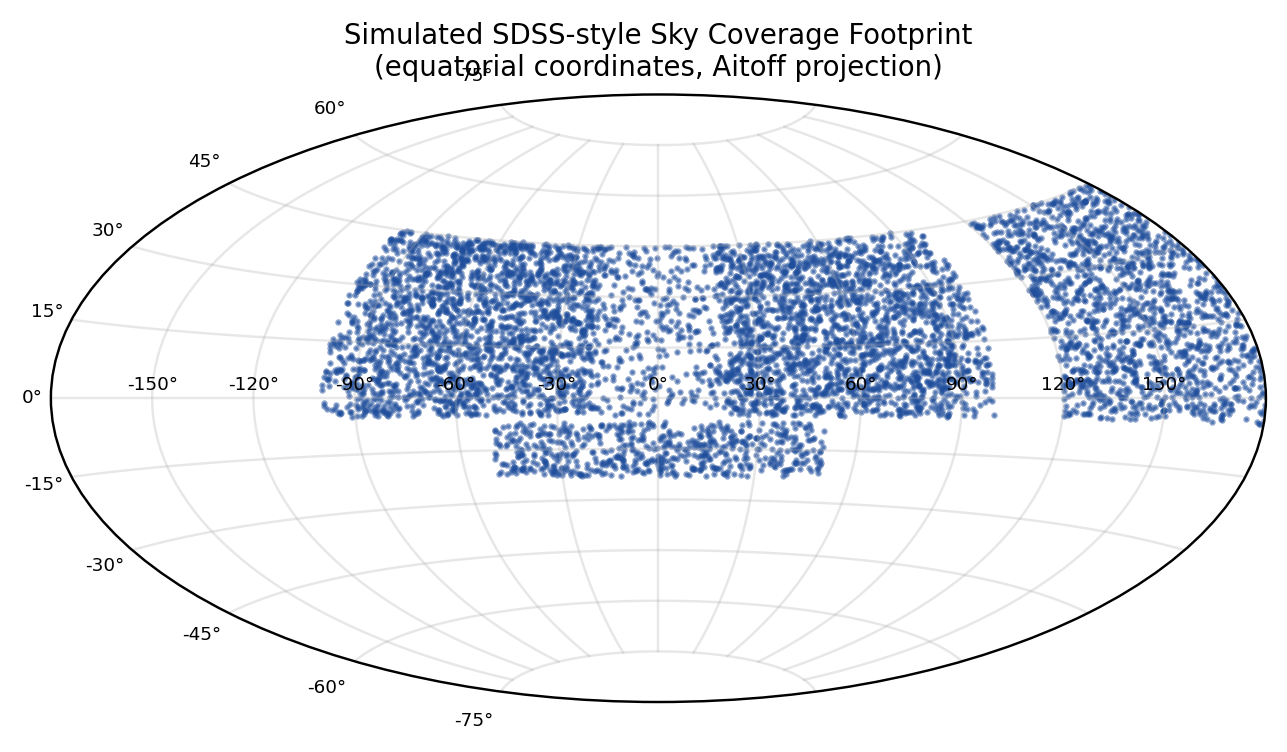
\includegraphics[width=0.72\textwidth]{sky_footprint.png}
  \caption{Illustrative sky coverage footprint in the style of an SDSS survey map (Aitoff projection, equatorial coordinates). Figure generated locally as a representative schematic; it is not an official SDSS data product.}
  \label{fig:sky-footprint}
\end{figure}

\begin{figure}[htbp]
  \centering
  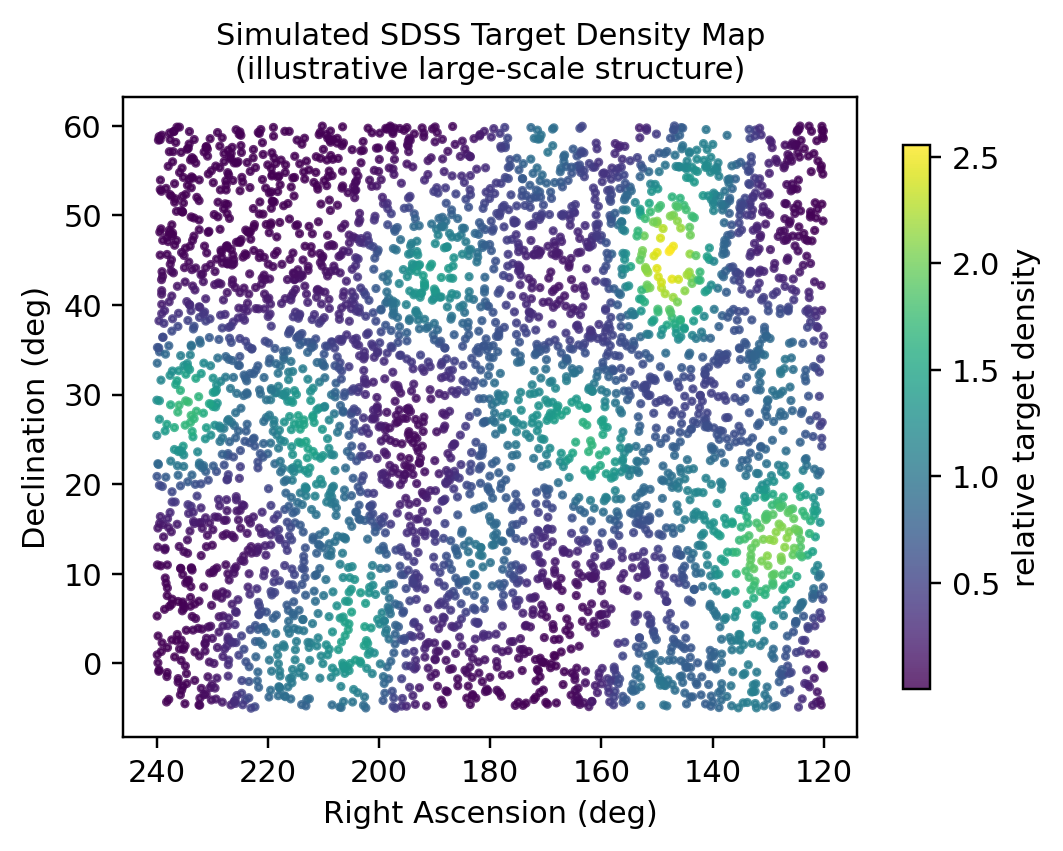
\includegraphics[width=0.62\textwidth]{sky_density.png}
  \caption{Illustrative target density map across right ascension and declination, showing the kind of large-scale structure visible in SDSS target catalogues. Figure generated locally as a representative schematic.}
  \label{fig:sky-density}
\end{figure}

\subsection{Software Libraries}

Four Python libraries form the backbone of the analysis pipeline:

\begin{itemize}[leftmargin=*]
  \item \textbf{Astropy} --- for general astronomy and astrophysics data handling, such as coordinate systems and FITS file I/O. \href{https://www.astropy.org}{astropy.org}
  \item \textbf{PyMultiFit} --- combines several functions for curve fitting. \href{https://github.com/syedalimohsinbukhari/pyMultiFit}{github.com/.../pyMultiFit}
  \item \textbf{NumPy} --- underlying numerical arrays and operations used throughout the pipeline. \href{https://numpy.org}{numpy.org}
  \item \textbf{Matplotlib} --- used to plot flux against wavelength and to generate the figures throughout this report. \href{https://matplotlib.org}{matplotlib.org}
\end{itemize}

\subsection{Initial Python Pipeline}

An initial Python pipeline was developed to open a spectrum FITS file and extract its data --- flux and wavelength (loglam) --- from the file. The extracted values were converted to standard units (\r{A}ngstr\"om for wavelength, and erg\,s$^{-1}$\,cm$^{-2}$\,\r{A}$^{-1}$ for flux). The code was then extended to plot flux against wavelength and mark/identify the various spectral lines within the plotted range, such as H$\alpha$, H$\beta$, and He\,I.

\begin{figure}[htbp]
  \centering
  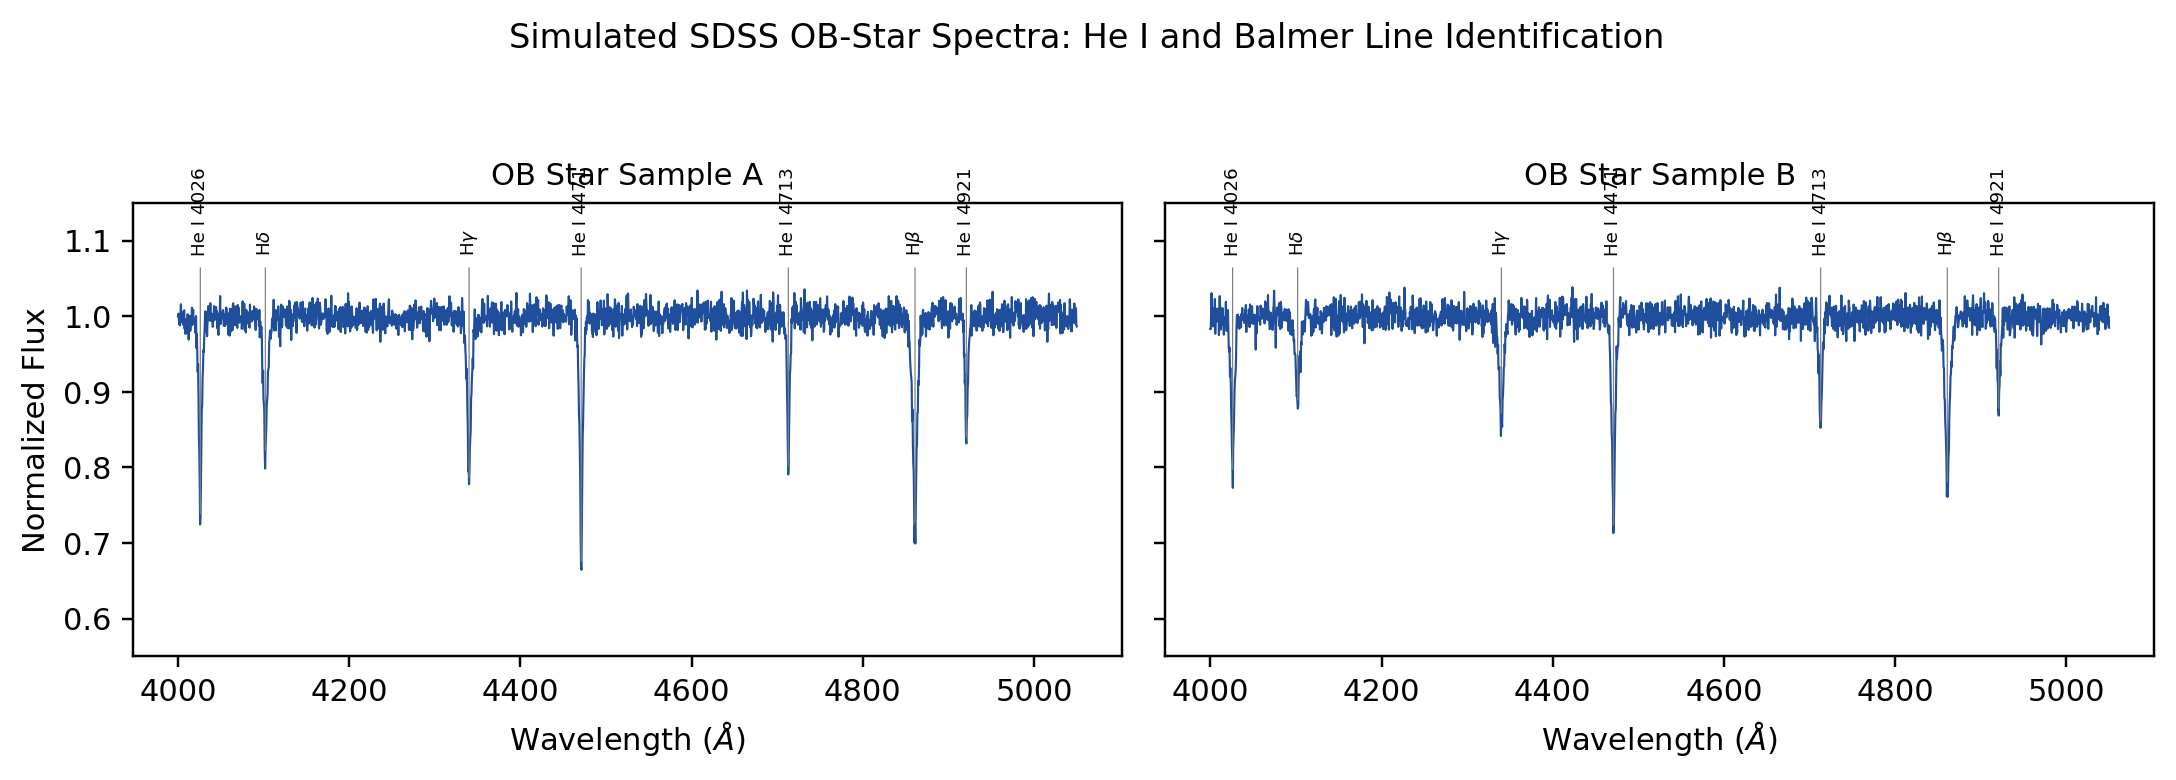
\includegraphics[width=\textwidth]{spectrum_grid.png}
  \caption{Simulated flux-versus-wavelength plots for two representative OB-type stellar spectra, with the He\,\textsc{i} and Balmer-series lines identified. Spectra are synthetically generated for illustration of the pipeline output; not drawn from real SDSS data.}
  \label{fig:spectrum-grid}
\end{figure}

\subsection{Equivalent Widths and Spectral Line Formation}

Spectral lines form through two basic interactions between light and matter:

\begin{itemize}[leftmargin=*]
  \item \textbf{Absorption:} atoms in a cooler gas absorb photons at precise wavelengths, exciting electrons to higher energy levels.
  \item \textbf{Emission:} electrons drop from an excited state back to the ground state, emitting photons with the same characteristic properties.
\end{itemize}

Ionization state matters for line identification: a \textbf{neutral} atom (e.g.\ He\,I) has had no electrons removed, so its lines arise from transitions within the neutral atom; a \textbf{singly ionized} atom (e.g.\ He\,II) has lost one electron. The hydrogen Balmer series is a useful reference ladder:

\begin{itemize}[leftmargin=*]
  \item H$\alpha$ ($n{=}3 \to n{=}2$) --- the strongest visible Balmer line.
  \item H$\beta$ ($n{=}4 \to n{=}2$) --- a strong diagnostic line.
  \item H$\gamma$ ($n{=}5 \to n{=}2$) --- comparatively weaker.
\end{itemize}

\paragraph{Equivalent width (EW).} The equivalent width is, in essence, the amount of light ``missing'' as a dip below the continuum: given a spectrum that follows a continuum (or a gentle slope) with a sudden dip, the EW is the width of a rectangle of the same area as that dip. Physically, it represents the interaction of light with the surrounding material at that specific wavelength:

\begin{itemize}[leftmargin=*]
  \item In \textbf{absorption}, EW reflects how many atoms are absorbing at that wavelength.
  \item In \textbf{emission}, EW reflects how much additional glowing gas is contributing to the light at that wavelength.
\end{itemize}

As a worked example from the literature: since a Be star such as $\zeta$~Tauri hosts a decretion disk, its H$\alpha$ EW --- measured relative to the star's own continuously emitted light --- traces how bright the disk's H$\alpha$ emission is. The reference paper measured this by integrating the flux above the continuum level between \SI{6520}{\angstrom} and \SI{6600}{\angstrom}: when the disk holds more gas the EW spikes, and as the disk thins the EW shrinks.

\subsection{Line Profile Shapes}

Three line-profile models were studied, each suited to a different physical regime:

\begin{enumerate}[leftmargin=*]
  \item \textbf{Lorentzian profile:} a tall, narrow-peaked shape caused by natural damping, collisions, and Stark broadening. Best suited to high-pressure environments and strong lines:
  \begin{equation}
    L(x) = \frac{\gamma/\pi}{(x - x_0)^2 + \gamma^2}
    \label{eq:lorentzian}
  \end{equation}
  \item \textbf{Gaussian profile:} bell-shaped and symmetric, caused by thermal broadening from the random motion of atoms. Best suited to weak lines:
  \begin{equation}
    G(x) = \frac{1}{\sigma\sqrt{2\pi}} \exp\!\left(-\frac{(x - x_0)^2}{2\sigma^2}\right)
    \label{eq:gaussian}
  \end{equation}
  where $x_0$ is the line centre and $\sigma$ is the standard deviation, related to the full width at half maximum by $\mathrm{FWHM} = 2\sqrt{2\ln 2}\,\sigma$.
  \item \textbf{Voigt profile:} a convolution of the Lorentzian and Gaussian profiles. Best suited to spectral lines in stars and plasmas:
  \begin{equation}
    V(x; \sigma, \gamma) = \int_{-\infty}^{\infty} G(x'; \sigma)\, L(x - x'; \gamma)\, dx' = \operatorname{Re}\!\left[\frac{w(z)}{\sigma\sqrt{2\pi}}\right],
    \quad z = \frac{(x - x_0) + i\gamma}{\sigma\sqrt{2}}
    \label{eq:voigt}
  \end{equation}
  where $G$ and $L$ are the Gaussian and Lorentzian profiles defined in \Cref{eq:gaussian,eq:lorentzian}, and $w(z)$ is the Faddeeva function, used in practice to evaluate the convolution efficiently.
\end{enumerate}

Direct integration of a line gives the true EW, but fitting one of the profiles above is what allows this to be measured accurately and consistently across many spectra.

\subsection{Line Ratios}

Line ratios compare the strength of two spectral lines: shared physical factors between the two lines cancel out, leaving only the differing factors, which can then be used to diagnose the physical conditions of the star. \Cref{tab:line-ratios} summarizes the diagnostic ratios studied this week.

% multirow

\begin{table}[htbp]
\centering
\caption{Diagnostic spectral line ratios and their physical interpretation.}
\label{tab:line-ratios}
\resizebox{\textwidth}{!}{
\begin{tabular}{@{}l p{0.64\textwidth} p{0.45\textwidth}@{}}
\toprule
\textbf{Ratio} & \textbf{Significance} & \textbf{Physical interpretation} \\
\midrule
\multirow{4}{*}{H$\alpha$ / H$\beta$}
  & \multirow{4}{0.28\textwidth}{Balmer decrement --- diagnoses dust extinction along the line of sight and flags non-standard emission (Be stars, active galaxies)}
  & $\approx 2.86$: normal, dust-free ionized gas (H\,\textsc{ii} regions, star-forming regions) \\
 & & $> 3$--4: dust absorbs more blue light, so H$\beta$ appears weaker \\
 & & $\geq 5$: very dust-polluted environments \\
 & & $< 2.86$: characteristic of Be stars or active galaxies \\
\addlinespace
He\,\textsc{ii} / He\,\textsc{i} & Traces the hardness of the ionizing radiation field & $> 0.82$: low in normal H\,\textsc{ii} regions, higher in hot, harder-radiation environments \\
\addlinespace
\ce{He+} / H$\beta$ & Flags sources of very high-energy ionizing photons & Low but significant values indicate a source capable of producing photons above \SI{54.4}{\eV} \\
\addlinespace
He\,\textsc{i} / H$\beta$ & Traces helium abundance & High values indicate high helium abundance \\
\addlinespace
\multirow{4}{*}{\ce{Fe+} / \ce{Fe}}
  & \multirow{4}{0.28\textwidth}{Diagnoses stellar effective temperature via the ionization balance of iron}
  & Small: cool stars (K, M); $T \approx \SIrange{5000}{5500}{\kelvin}$ \\
 & & Moderate: G-type stars; $T \approx \SIrange{5500}{6000}{\kelvin}$ \\
 & & High: F- and A-type stars; $T \approx \SIrange{6000}{8000}{\kelvin}$ \\
 & & Very high: early B-type stars; higher temperature, lower surface gravity \\
\bottomrule
\end{tabular}
}
\end{table}

\subsection{Fitter Development}

Development then moved from theory to code. A Gaussian fitter was written first, followed by a Lorentzian fitter --- structurally very similar, differing mainly in the amplitude formula. Since \texttt{PyMultiFit} does not natively support negative-amplitude (absorption-dip) fits, an additional class was written to hold negative amplitude parameters, producing plots with both positive and negative peaks. The same adjustment was needed for the Lorentzian case; since PyMultiFit did not include a default Lorentzian fitter at all, this required writing the base Lorentzian fitter from scratch before adding the negative-amplitude extension. The final days of Week 1 focused on studying how a zero-centered distribution is adjusted to match a star's spectrum (which sits at some nonzero baseline $y$-value), and revisiting what EWs and spectral dips represent physically.


\section{Theoretical Background: OB Stars}
\label{sec:theory}

OB stars are among the hottest and most massive stars on the main sequence, with effective surface temperatures typically ranging from roughly \SI{10000}{\kelvin} to over \SI{30000}{\kelvin}. At these temperatures, hydrogen is largely ionized in the stellar photosphere, which suppresses the strength of the Balmer series relative to cooler stars, while neutral helium (\ce{He}) transitions become strong and are often the dominant absorption features in the optical spectrum. This is precisely the pattern observed in the sample analysed here: the \ce{He} series ($\lambda \approx \SIlist{4026;4471;4713;4921;5015;5876}{\angstrom}$, among others) appears almost universally, while hydrogen features are comparatively weak, blended, or absent.

Absorption lines form when photons emerging from the deeper, hotter layers of a star are absorbed by atoms and ions in the cooler outer photosphere, at wavelengths corresponding to the energy difference between two electronic states of that species. The depth, width, and shape of each absorption feature (the ``line profile'') encode physical information about the star, including its temperature, surface gravity, rotational velocity, and chemical composition. Fitting these profiles mathematically, as introduced in \Cref{sec:background}, is therefore a key step in quantitative spectroscopy.




\end{document}